\mode*

\begin{frame}[fragile]{La cohérence séquentielle}

\vfill
\begin{center}
   \alert{Quand peut-on dire qu'une implémentation est \alert{correcte} ?}
\end{center}    

\vfill
\begin{block}{Rappels}
  \begin{itemize}
  \item Raisonnements sur les exécutions à base d'\structure{entrelacements}
  \item Nécessite des exécutions \structure{séquentiellement cohérentes}
  \end{itemize}
\end{block}
\vfill

\begin{block}{Exécution séquentiellement cohérente}
  Le résultat observable d'une exécution est le même que celui d'un entrelacement de l'ordre ``happened before''
\end{block}

\pause

\vfill
\begin{block}{Objet partagé séquentiellement cohérent}
  Le résultat observable \alert{des opérations sur l'objet partagé} d'une exécution est le même que celui d'un entrelacement de l'ordre ``happened before''
\end{block}
\vfill

\end{frame}

\begin{frame}[fragile]{Composabilité des critères de cohérence}
    \begin{lstlisting}[numbers=none]
public static void main(String[] args) {    
  var x = new SequentiallyConsistentCounter(0);
  var y = new SequentiallyConsistentCounter(0);
   
  new Thread(() ->
    x.increment();
    System.out.print(y.get());
  ).start();
   
  new Thread(() ->
    y.increment();
    System.out.print(x.get());
  ).start();
}
    \end{lstlisting}

\vspace{-3mm}
\begin{center}
  \color{exampleColor} Quelles sont les sorties possibles ? 
\end{center}
\pause
\begin{block}{Composabilité}
   \begin{itemize}
      \item Si deux objets sont cohérents, leur composition est cohérente 
      \item \alert{La cohérence séquentielle n'est pas composable !}
   \end{itemize}
\end{block}
\end{frame}


\begin{frame}{Linéarisabilité}
  \vFill
  \hFill
  \begin{minipage}{.6\textwidth}
    \begin{center}
      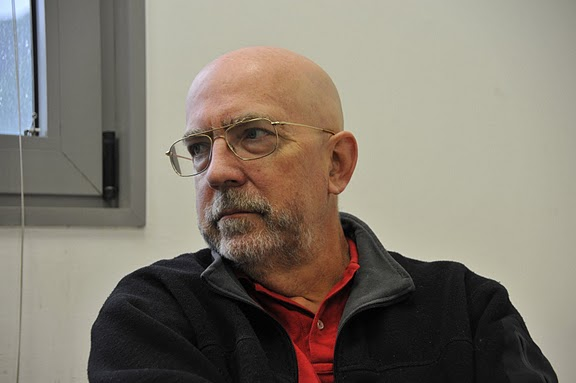
\includegraphics[height=4cm]{Herlihy}\\
      Maurice P. Herlihy
    \end{center}
  \end{minipage}
  \hFill
  \begin{minipage}{.28\textwidth}
    \begin{center}
      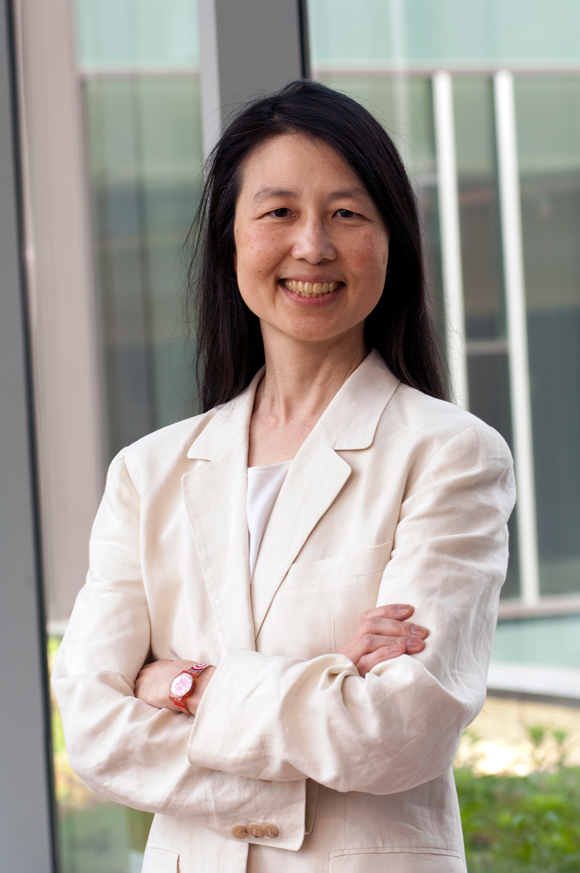
\includegraphics[height=4cm]{Wing}\\
      Jeanette M. Wing
    \end{center}
  \end{minipage}
  \hFill

  \vFill
  \begin{citing}
  \item[L86] Leslie Lamport. \textit{On interprocess communication.} Distributed Computing (1986)
  \item[HW90] Maurice P. Herlihy, Jeanette M. Wing. \textit{Linearizability: A Correctness Condition for Concurrent Objects.} ToPLaS (1990)
  \end{citing}
\end{frame}




\begin{frame}{Linéarisabilité}
  \begin{block}{Définition}
    Un objet partagé est linéarisable si : \\
    le résultat observable des opérations sur l'objet partagé d'une exécution est le même que celui d'un entrelacement de l'ordre ``happened before''
    \alert{tel que, si une opération $e$ se termine avant qu'une autre opération $e'$ ne commence, alors $e$ doit précéder $e'$ dans l'entrelacement}
  \end{block}

\vfill
  \begin{exampleblock}{Exemple}
  \vspace{-3mm}
    \begin{center}
    \scalebox{.7}{
      \begin{tikzpicture}
        \draw[-latex] (0,3) node[left]{$T_1$} -- (10,3);
        \draw[-latex] (0,2) node[left]{$T_2$} -- (10,2);

        \draw[exampleColor, fill=exampleColor!20, rounded corners] (1 , 1.6) rectangle (5 , 2.4);
        \draw[exampleColor, fill=exampleColor!20, rounded corners] (6, 2.6) rectangle (9, 3.4);

        \draw[exampleColor] (3,2) node{$increment()$ };
        \draw[exampleColor] (7.5,3) node{$get()$};
        \end{tikzpicture}
    }
    \end{center}

    Un seul ordre de linéarisation possible : 
    \begin{itemize}
    \item $increment() ;~ get()$
      \begin{itemize}
      \item La lecture doit retourner 1
      \end{itemize}
    \end{itemize}
  \end{exampleblock}

\end{frame}

\begin{frame}{Caractérisation}

  \begin{block}{Point de linéarisation}
    Un objet partagé est linéarisable si, et seulement si : \\
    le résultat observable des opérations sur l'objet partagé d'une exécution est le même que si
    \alert{chaque opération avait lieu en un point atomique
    situé entre son début et sa fin.}
  \end{block}

  \vfill
  \begin{exampleblock}{Exemple}

\begin{center}
    \scalebox{.7}{
      \begin{tikzpicture}
        \draw[exampleColor, -latex] (0,4) node[left]{$counter$} -- (10,4);
        \draw[-latex] (0,3) node[left]{$T_1$} -- (10,3);
        \draw[-latex] (0,2) node[left]{$T_2$} -- (10,2);

        \draw[exampleColor, thick, densely dotted] (3  , 2) -- (3  , 4) node{$\bullet$};
        \draw[exampleColor, thick, densely dotted] (7.5, 3) -- (7.5, 4) node{$\bullet$};

        \draw[exampleColor, fill=exampleColor!20, rounded corners] (1 , 1.6) rectangle (5 , 2.4);
        \draw[exampleColor, fill=exampleColor!20, rounded corners] (6, 2.6) rectangle (9, 3.4);

        \draw[exampleColor] (3,2) node{$increment()$ };
        \draw[exampleColor] (7.5,3) node{$get()$};
        \end{tikzpicture}
    }
    \end{center}
  \end{exampleblock}

\vfill
\small
  \begin{alertblock}{Propriétés}
  \vspace{-2mm}
    \begin{itemize}
      \item La linéarisabilité est composable
      \item La linéarisabilité implique la cohérence séquentielle
      \item Si chaque objet est linéarisable, l'exécution est séquentiellement cohérente
    \end{itemize}
  \end{alertblock}
\end{frame}

\begin{frame}[fragile]{Exemple}
\vspace{-3mm}
\begin{center}
\scalebox{.6}{
      \begin{tikzpicture}
        \draw[white] (-2.5,0.5) rectangle (15,4);

        \draw[structure ,     -latex] (-1,3) node[left]{$T_1$} -- (15,3);
        \draw[exampleColor,   -latex] (-1,2) node[left]{$T_2$} -- (15,2);
        \draw<7> [alertColor, -latex] (-1,1) node[left]{$result$} +(.2,.15) node{$0$} +(0,0) -- (15,1);
        \draw<2-6>[alertColor, -latex] (-1,1) node[left]{$counter$} +(.2,.15) node{$0$} +(0,0) -- (15,1);

        \draw[exampleColor, fill=exampleColor!20, rounded corners] (1 , 1.6) rectangle (5 , 2.4);
        \draw[exampleColor, fill=exampleColor!20, rounded corners] (6 , 1.6) rectangle (13, 2.4);
        \draw[structure, fill=structure!20, rounded corners] (2 , 2.6) rectangle (10, 3.4);
        \draw[structure, fill=structure!20, rounded corners] (11, 2.6) rectangle (14, 3.4);

        \draw<7>[alertColor, fill=alertColor!20, rounded corners] (1.1 , 1.7) rectangle (2.9 , 2.3);
        \draw<7>[alertColor, fill=alertColor!20, rounded corners] (3.1 , 1.7) rectangle (4.9 , 2.3);
        \draw<7>[alertColor, fill=alertColor!20, rounded corners] (6.1 , 1.7) rectangle (12.9, 2.3);
        \draw<7>[alertColor, fill=alertColor!20, rounded corners] (2.1 , 2.7) rectangle (5.4, 3.3);
        \draw<7>[alertColor, fill=alertColor!20, rounded corners] (5.6 , 2.7) rectangle (9.9, 3.3);
        \draw<7>[alertColor, fill=alertColor!20, rounded corners] (11.1, 2.7) rectangle (13.9, 3.3);

        \draw<7>[alertColor] (2   , 2) node{$get()$}; 
        \draw<7>[alertColor] (4   , 2) node{$put(1)$}; 
        \draw<7>[alertColor] (9.5 , 2) node{$get()$}; 
        \draw<7>[alertColor] (4.25, 3) node{$get()$}; 
        \draw<7>[alertColor] (7.75, 3) node{$put(1)$}; 
        \draw<7>[alertColor] (12.5, 3) node{$get()$}; 

        \draw<7>[alertColor, thick, densely dotted] (2   , 1.7) -- (2   , 1) node{$\bullet$} ++(0,.15) node[right]{\footnotesize$0$}; 
        \draw<7>[alertColor, thick, densely dotted] (4   , 1.7) -- (4   , 1) node{$\bullet$} ++(0,.15) node[right]{\footnotesize$1$}; 
        \draw<7>[alertColor, thick, densely dotted] (9.5 , 1.7) -- (9.5 , 1) node{$\bullet$} ++(0,.15) node[right]{\footnotesize$1$}; 
        \draw<7>[alertColor, thick, densely dotted] (3, 2.7)    -- (3, 1)    node{$\bullet$} ++(0,.15) node[right]{\footnotesize$0$}; 
        \draw<7>[alertColor, thick, densely dotted] (7.75, 2.7) -- (7.75, 1) node{$\bullet$} ++(0,.15) node[right]{\footnotesize$1$}; 
        \draw<7>[alertColor, thick, densely dotted] (12.5, 2.7) -- (12.5, 1) node{$\bullet$} ++(0,.15) node[right]{\footnotesize$1$}; 

        \draw<7>[structure] (6,3.65) node{$increment()$ };
        \draw<7>[structure] (12.5,3.65) node{$get()$};
        \draw<7>[exampleColor] (1,1.35) node{$increment()$ };
        \draw<7>[exampleColor] (11,1.35) node{$get()$};

        \draw<-6>[structure] (6,3) node{$increment()$ };
        \draw<1>[structure] (12.5,3) node{$get()$};
        \draw<2>[structure] (12.5,3) node{$get()$ retourne $2$};
        \draw<3>[structure] (12.5,3) node{$get()$ retourne $2$};
        \draw<4>[structure] (12.5,3) node{$get()$ retourne $2$};
        \draw<5>[structure] (12.5,3) node{$get()$ retourne $2$};
        \draw<6>[structure] (12.5,3) node{$get()$ retourne $2$};
        \draw<-6>[exampleColor] (3,2) node{$increment()$ };
        \draw<1>[exampleColor] (9.5,2) node{$get()$};
        \draw<2>[exampleColor] (9.5,2) node{$get()$ retourne $2$};
        \draw<3>[exampleColor] (9.5,2) node{$get()$ retourne $2$};
        \draw<4>[exampleColor] (9.5,2) node{$get()$ retourne $2$};
        \draw<5>[exampleColor] (9.5,2) node{$get()$ retourne $2$};
        \draw<6>[exampleColor] (9.5,2) node{$get()$ retourne $1$};

        \draw<2>[densely dotted, thick, structure]    (4.0  ,2.6) node{$\bullet$} -- (4.0  ,1)    node{$\bullet$};
        \draw<2>[densely dotted, thick, structure]    (11.5 ,2.6) node{$\bullet$} -- (11.5 ,1) node{$\bullet$};
        \draw<2>[densely dotted, thick, exampleColor] (4.5  ,1.6) node{$\bullet$} -- (4.5  ,1)    node{$\bullet$};
        \draw<2>[densely dotted, thick, exampleColor] (12.5 ,1.6) node{$\bullet$} -- (12.5 ,1)  node{$\bullet$};

        \draw<3>[densely dotted, thick, structure]    (4.0  ,2.6) node{$\bullet$} -- (4.0  ,1)    node{$\bullet$};
        \draw<3>[densely dotted, thick, structure]    (13.5 ,2.6) node{$\bullet$} -- (13.5 ,1) node{$\bullet$};
        \draw<3>[densely dotted, thick, exampleColor] (4.5  ,1.6) node{$\bullet$} -- (4.5  ,1)    node{$\bullet$};
        \draw<3>[densely dotted, thick, exampleColor] (9.5  ,1.6) node{$\bullet$} -- (9.5  ,1)  node{$\bullet$};

        \draw<4>[densely dotted, thick, structure]    (5.5  ,2.6) node{$\bullet$} -- (5.5  ,1)    node{$\bullet$};
        \draw<4>[densely dotted, thick, structure]    (11.5 ,2.6) node{$\bullet$} -- (11.5 ,1) node{$\bullet$};
        \draw<4>[densely dotted, thick, exampleColor] (3    ,1.6) node{$\bullet$} -- (3    ,1)    node{$\bullet$};
        \draw<4>[densely dotted, thick, exampleColor] (12.5 ,1.6) node{$\bullet$} -- (12.5  ,1)  node{$\bullet$};

        \draw<5>[densely dotted, thick, structure]    (5.5  ,2.6) node{$\bullet$} -- (5.5  ,1)    node{$\bullet$};
        \draw<5>[densely dotted, thick, structure]    (13.5 ,2.6) node{$\bullet$} -- (13.5 ,1) node{$\bullet$};
        \draw<5>[densely dotted, thick, exampleColor] (3    ,1.6) node{$\bullet$} -- (3    ,1)    node{$\bullet$};
        \draw<5>[densely dotted, thick, exampleColor] (9.5  ,1.6) node{$\bullet$} -- (9.5  ,1)  node{$\bullet$};

        \draw<6>[densely dotted, thick, structure]    (7.5  ,2.6) node{$\bullet$} -- (7.5  ,1)    node{$\bullet$};
        \draw<6>[densely dotted, thick, structure]    (13.5 ,2.6) node{$\bullet$} -- (13.5 ,1) node{$\bullet$};
        \draw<6>[densely dotted, thick, exampleColor] (3    ,1.6) node{$\bullet$} -- (3    ,1)    node{$\bullet$};
        \draw<6>[densely dotted, thick, exampleColor] (6.5  ,1.6) node{$\bullet$} -- (6.5  ,1)  node{$\bullet$};


\end{tikzpicture}
}
\end{center}
\pause
\begin{alertblock}{Linéarisations acceptables}
      \begin{itemize}
      \item $\structure{T_1:increment();}~{\color{exampleColor}T_2:increment();}~\structure{T_1:get();}~{\color{exampleColor}T_2:get();}$
        \begin{itemize}
        \item Les deux lectures retournent 2
        \end{itemize}
        \pause
      \item $\structure{T_1:increment();}~{\color{exampleColor}T_2:increment();}~{\color{exampleColor}T_2:get();}~\structure{T_1:get();}$
        \begin{itemize}
        \item Les deux lectures retournent 2
        \end{itemize}
        \pause
      \item ${\color{exampleColor}T_2:increment();}~\structure{T_1:increment();}~\structure{T_1:get();}~{\color{exampleColor}T_2:get();}$
        \begin{itemize}
        \item Les deux lectures retournent 2
        \end{itemize}
        \pause
      \item ${\color{exampleColor}T_2:increment();}~\structure{T_1:increment();}~{\color{exampleColor}T_2:get();}~\structure{T_1:get();}$
        \begin{itemize}
        \item Les deux lectures retournent 2
        \end{itemize}
        \pause
      \item ${\color{exampleColor}T_2:increment();}~{\color{exampleColor}T_2:get();}~\structure{T_1:increment();}~\structure{T_1:get();}$
        \begin{itemize}
        \item $T_1$ lit $2$ et $T_2$ lit $1$
        \end{itemize}
      \end{itemize}
      \end{alertblock}
%    \end{itemize}

\end{frame}





\begin{frame}{Algorithmes d'incrémentation}
\begin{block}{Algorithme bloquant}
\begin{itemize}
\item Point de linéarisation n'importe où en section critique
\end{itemize}
\centering
\scalebox{.6}{\begin{tikzpicture}
        \draw[exampleColor, fill=exampleColor!20, rounded corners] (0.6,0.6)  rectangle (10.1,1.4);
        \draw[alertColor, fill=alertColor!20, rounded corners] (0.6,-0.4) rectangle (5.8,0.4);
 
        \draw[structure, -latex] (0,2) node[left]{$counter$} +(.2,.15) node{$0$} +(0,0) -- (10.5,2);
        \draw[exampleColor,-latex] (0,1) node[left]{$t1$} -- (10.5,1);
        \draw[alertColor, -latex] (0,0) node[left]{$t2$} -- (10.5,0);
        \draw[structure, -latex] (0,-1   ) node[left]{\scriptsize $value$} +(.15,.12) node{\scriptsize $0$} +(0,0) -- (10.5,-1   );
        \draw[structure, -latex] (0,-1.25) node[left]{\scriptsize $lock$}  +(0,0) -- (10.5,-1.25);
 
        \draw[exampleColor, thick, densely dotted] (7.9 ,1.4) node{$\bullet$} -- (7.9 ,2) node{$\bullet$} ++(0,.15) node[left]{\footnotesize$increment()$} node[right]{\footnotesize$2$}; 
        \draw[alertColor,   thick, densely dotted] (3.6 ,0.4) node{$\bullet$} -- (3.6 ,2) node{$\bullet$} ++(0,.15) node[left]{\footnotesize$increment()$} node[right]{\footnotesize$1$}; 
 
        \draw[alertColor,   ultra thick] (1.2 ,-1.25) -- (5.0 ,-1.25) ; 
        \draw[exampleColor, ultra thick] (5.75 ,-1.25) -- (9.3 ,-1.25) ; 
 
 
        \draw[structure, thick, densely dotted] (5.75 ,1) -- (5.75 ,-1.25) node{$\bullet$} +(.15,.12) ; 
        \draw[structure, thick, densely dotted] (6.7 ,1) -- (6.7 ,-1   ) node{$\bullet$} +(.15,.12) node{\scriptsize $1$}; 
        \draw[structure, thick, densely dotted] (7.9 ,1) -- (7.9 ,-1   ) node{$\bullet$} +(.15,.12) node{\scriptsize $2$}; 
        \draw[structure, thick, densely dotted] (9.3 ,1) -- (9.3 ,-1.25) node{$\bullet$} +(.15,.12) ; 
        \draw[structure, thick, densely dotted] (1.2 ,0) -- (1.2 ,-1.25) node{$\bullet$} +(.15,.12) ; 
        \draw[structure, thick, densely dotted] (2.4 ,0) -- (2.4 ,-1   ) node{$\bullet$} +(.15,.12) node{\scriptsize $0$}; 
        \draw[structure, thick, densely dotted] (3.6 ,0) -- (3.6 ,-1   ) node{$\bullet$} +(.15,.12) node{\scriptsize $1$}; 
        \draw[structure, thick, densely dotted] (5.0 ,0) -- (5.0 ,-1.25) node{$\bullet$} +(.15,.12) ; 
 
 
        \draw[structure, fill=structure!20, rounded corners] (3.0 ,1)  +(-2.3,-0.3) rectangle +(3.0,0.3) +(0,0) node{$lock()$};
        \draw[structure, fill=structure!20, rounded corners] (6.7 ,1)  +(-0.5,-0.3) rectangle +(0.5,0.3) +(0,0) node{$get()$};
        \draw[structure, fill=structure!20, rounded corners] (7.9 ,1)  +(-0.5,-0.3) rectangle +(0.5,0.3) +(0,0) node{$set(2)$};
        \draw[structure, fill=structure!20, rounded corners] (9.3 ,1)  +(-0.7,-0.3) rectangle +(0.7,0.3) +(0,0) node{$unlock()$};
        \draw[structure, fill=structure!20, rounded corners] (1.2 ,0)  +(-0.5,-0.3) rectangle +(0.5,0.3) +(0,0) node{$lock()$};
        \draw[structure, fill=structure!20, rounded corners] (2.4 ,0)  +(-0.5,-0.3) rectangle +(0.5,0.3) +(0,0) node{$get()$};
        \draw[structure, fill=structure!20, rounded corners] (3.6 ,0)  +(-0.5,-0.3) rectangle +(0.5,0.3) +(0,0) node{$set(1)$};
        \draw[structure, fill=structure!20, rounded corners] (5.0 ,0)  +(-0.7,-0.3) rectangle +(0.7,0.3) +(0,0) node{$unlock()$};
 
 
        \end{tikzpicture}}
        \end{block}
\begin{block}{Algorithme non-bloquant}
\begin{itemize}
\item Point de linéarisation sur la dernière instruction \lstinline{compareAndSet} 
\end{itemize}
\centering
   \scalebox{.6}{\begin{tikzpicture}
        \draw[exampleColor, fill=exampleColor!20, rounded corners] (0.6,0.6)  rectangle (10.1,1.4);
        \draw[alertColor, fill=alertColor!20, rounded corners] (0.6,-0.4) rectangle (5.8,0.4);
 
        \draw[structure, -latex] (0,2) node[left]{$counter$} +(.2,.15) node{$0$} +(0,0) -- (10.5,2);
        \draw[exampleColor,-latex] (0,1) node[left]{$t1$} -- (10.5,1);
        \draw[alertColor, -latex] (0,0) node[left]{$t2$} -- (10.5,0);
        \draw[structure, -latex] (0,-1   ) node[left]{\scriptsize $value$} +(.15,.12) node{\scriptsize $0$} +(0,0) -- (10.5,-1   );
 
        \draw[exampleColor, thick, densely dotted] (8.0 ,1.4) node{$\bullet$} -- (8.0 ,2) node{$\bullet$} ++(0,.15) node[left]{\footnotesize$increment()$} node[right]{\footnotesize$2$}; 
        \draw[alertColor,   thick, densely dotted] (4.0 ,0.4) node{$\bullet$} -- (4.0 ,2) node{$\bullet$} ++(0,.15) node[left]{\footnotesize$increment()$} node[right]{\footnotesize$1$};  
 
        \draw[structure, thick, densely dotted] (8.0 ,1) -- (8.0 ,-1) node{$\bullet$} +(.15,.12) node{\scriptsize $2$}; 
        \draw[structure, thick, densely dotted] (4.0 ,0) -- (4.0 ,-1) node{$\bullet$} +(.15,.12) node{\scriptsize $1$}; 
        \draw[structure, thick, densely dotted] (3.0 ,1) -- (3.0 ,-1) node{$\bullet$};
        \draw[structure, thick, densely dotted] (5.0 ,1) -- (5.0 ,-1) node{$\bullet$};
        \draw[structure, thick, densely dotted] (6.5 ,1) -- (6.5 ,-1) node{$\bullet$};
        \draw[structure, thick, densely dotted] (2.0 ,0) -- (2.0 ,-1) node{$\bullet$};


        \draw[structure, fill=structure!20, rounded corners] (3.0 ,1)  +(-0.50,-0.3) rectangle +(0.50,0.3) +(0,0) node{$get()$};
        \draw[structure, fill=structure!20, rounded corners] (5.0 ,1)  +(-0.75,-0.3) rectangle +(0.75,0.3) +(0,0) node{$cas(0, 1)$};
        \draw[structure, fill=structure!20, rounded corners] (6.5 ,1)  +(-0.50,-0.3) rectangle +(0.50,0.3) +(0,0) node{$get()$};
        \draw[structure, fill=structure!20, rounded corners] (8.0 ,1)  +(-0.75,-0.3) rectangle +(0.75,0.3) +(0,0) node{$cas(1, 2)$};
        \draw[structure, fill=structure!20, rounded corners] (2.0 ,0)  +(-0.50,-0.3) rectangle +(0.50,0.3) +(0,0) node{$get()$};
        \draw[structure, fill=structure!20, rounded corners] (4.0 ,0)  +(-0.75,-0.3) rectangle +(0.75,0.3) +(0,0) node{$cas(0, 1)$};
 
        \end{tikzpicture}}
        \end{block}
\end{frame}



\mode<all>


